\section{Desenvolvimento}
	
	Conforme o supracitado, o presente estuda visa o desenvolvimento de uma plataforma de jogo, adaptando o jogo "Pong" para tecnologias mais recentes. Inicialmente, para que hajam menos complicações eventuais, é primordial entender o funcionamento do jogo e suas características.

\begin{figure}[htbp]
     \centerline{
        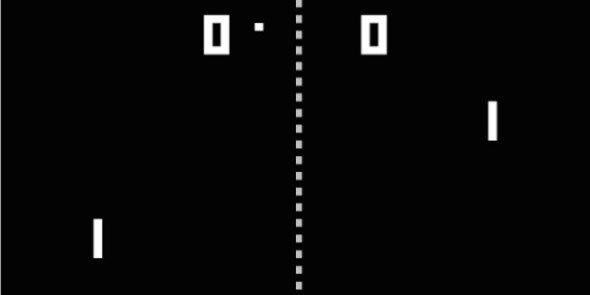
\includegraphics[width=3in]{pong-exemplo.jpg}
        }
     \caption{Exemplo de como é o jogo "Pong".}
     \label{fig}
    \end{figure}

	O "Pong" é uma simulação de uma partida de tênis de mesa vista de cima, com alguns objetos que compõem a tela: duas barras, sendo uma para cada jogador, uma bola que ficará andando pela tela e o placar, com a pontuação de cada jogador respectivamente. O objetivo do jogo é que o jogador, controlando uma das barras, impeça a bola de bater no seu lado, somando pontos fazendo a bola chegar do outro lado sem que o oponente consiga "defender". As barras tem movimento unidimensional que pode ser controlado por um pequeno joystick composto por um reostato ou potenciômetro.

	Como o projeto não envolve apenas o jogo, mas os controles deste, que utilizarão botões e potenciômetros, o primeiro passo será efetuar a integração desses com o Arduino UNO através do simulador virtual TinkerCAD, visando uma segurança maior e a garantia de que nenhum componente falhe durante a construção do Hardware.

	Com isso, estabelecer uma comunicação entre o Processing e o Arduino é fundamental, já que as informações coletadas dos botões e potenciômetros devem passar de um para o outro. Essa comunicação será possível através do modelo serial, já que ambos podem enviar e receber informações por esse modelo com suas respectivas bibliotecas específicas e para que isso ocorra, basta utilizar o cabo USB do próprio microcontrolador e associar a porta a qual este está conectado ao Processing, garantindo que essas informações sejam enviadas. Isso ocorre de maneira mais simples por se tratar de uma comunicação Arduino-computador ao invés de dois microcontroladores diferentes, sem necessidade de utilizar métodos como o "Protocolo UART" nessa situação.
	
	Em se tratando do jogo, que será programado na liguagem Processing, que é notadamente baseada em noções de "C" e "Java". Além do próprio "Pong", o jogo contará com uma tela de início, um menu com as instruções e uma tela de pause. Por ser uma linguagem de ambiente de desenvolvimento integrado (IDE), Processing se mostra apropriado para desenvolvimento de um jogo. A utilização de "classes" tangentes a da linguagem "Java" por exemplo, é uma maneira muito eficaz de se criar objetos dinâmicos que integram o jogo, como as barras e a bola. Por definição, as classes são um conjunto de atributos e métodos que podem ser instanciados por objetos, abstraindo-os.

